\section{Introduction}\label{sec:intro}

Text-to-motion generation has made striking progress, but almost all of it on
one body. The standard pipeline---a diffusion model, a motion tokenizer or a
latent generator trained on HumanML3D~\citep{guo2022generating}---assumes a
fixed kinematic tree, typically the 22-joint SMPL skeleton, and bakes that
assumption into every layer: the input projection has a fixed joint count,
positional encodings index fixed joint slots, and any codebook is learned for
one morphology. The result is a family of models that are excellent at
animating a human and structurally unable to animate anything else.

\begin{figure}[t]
\centering
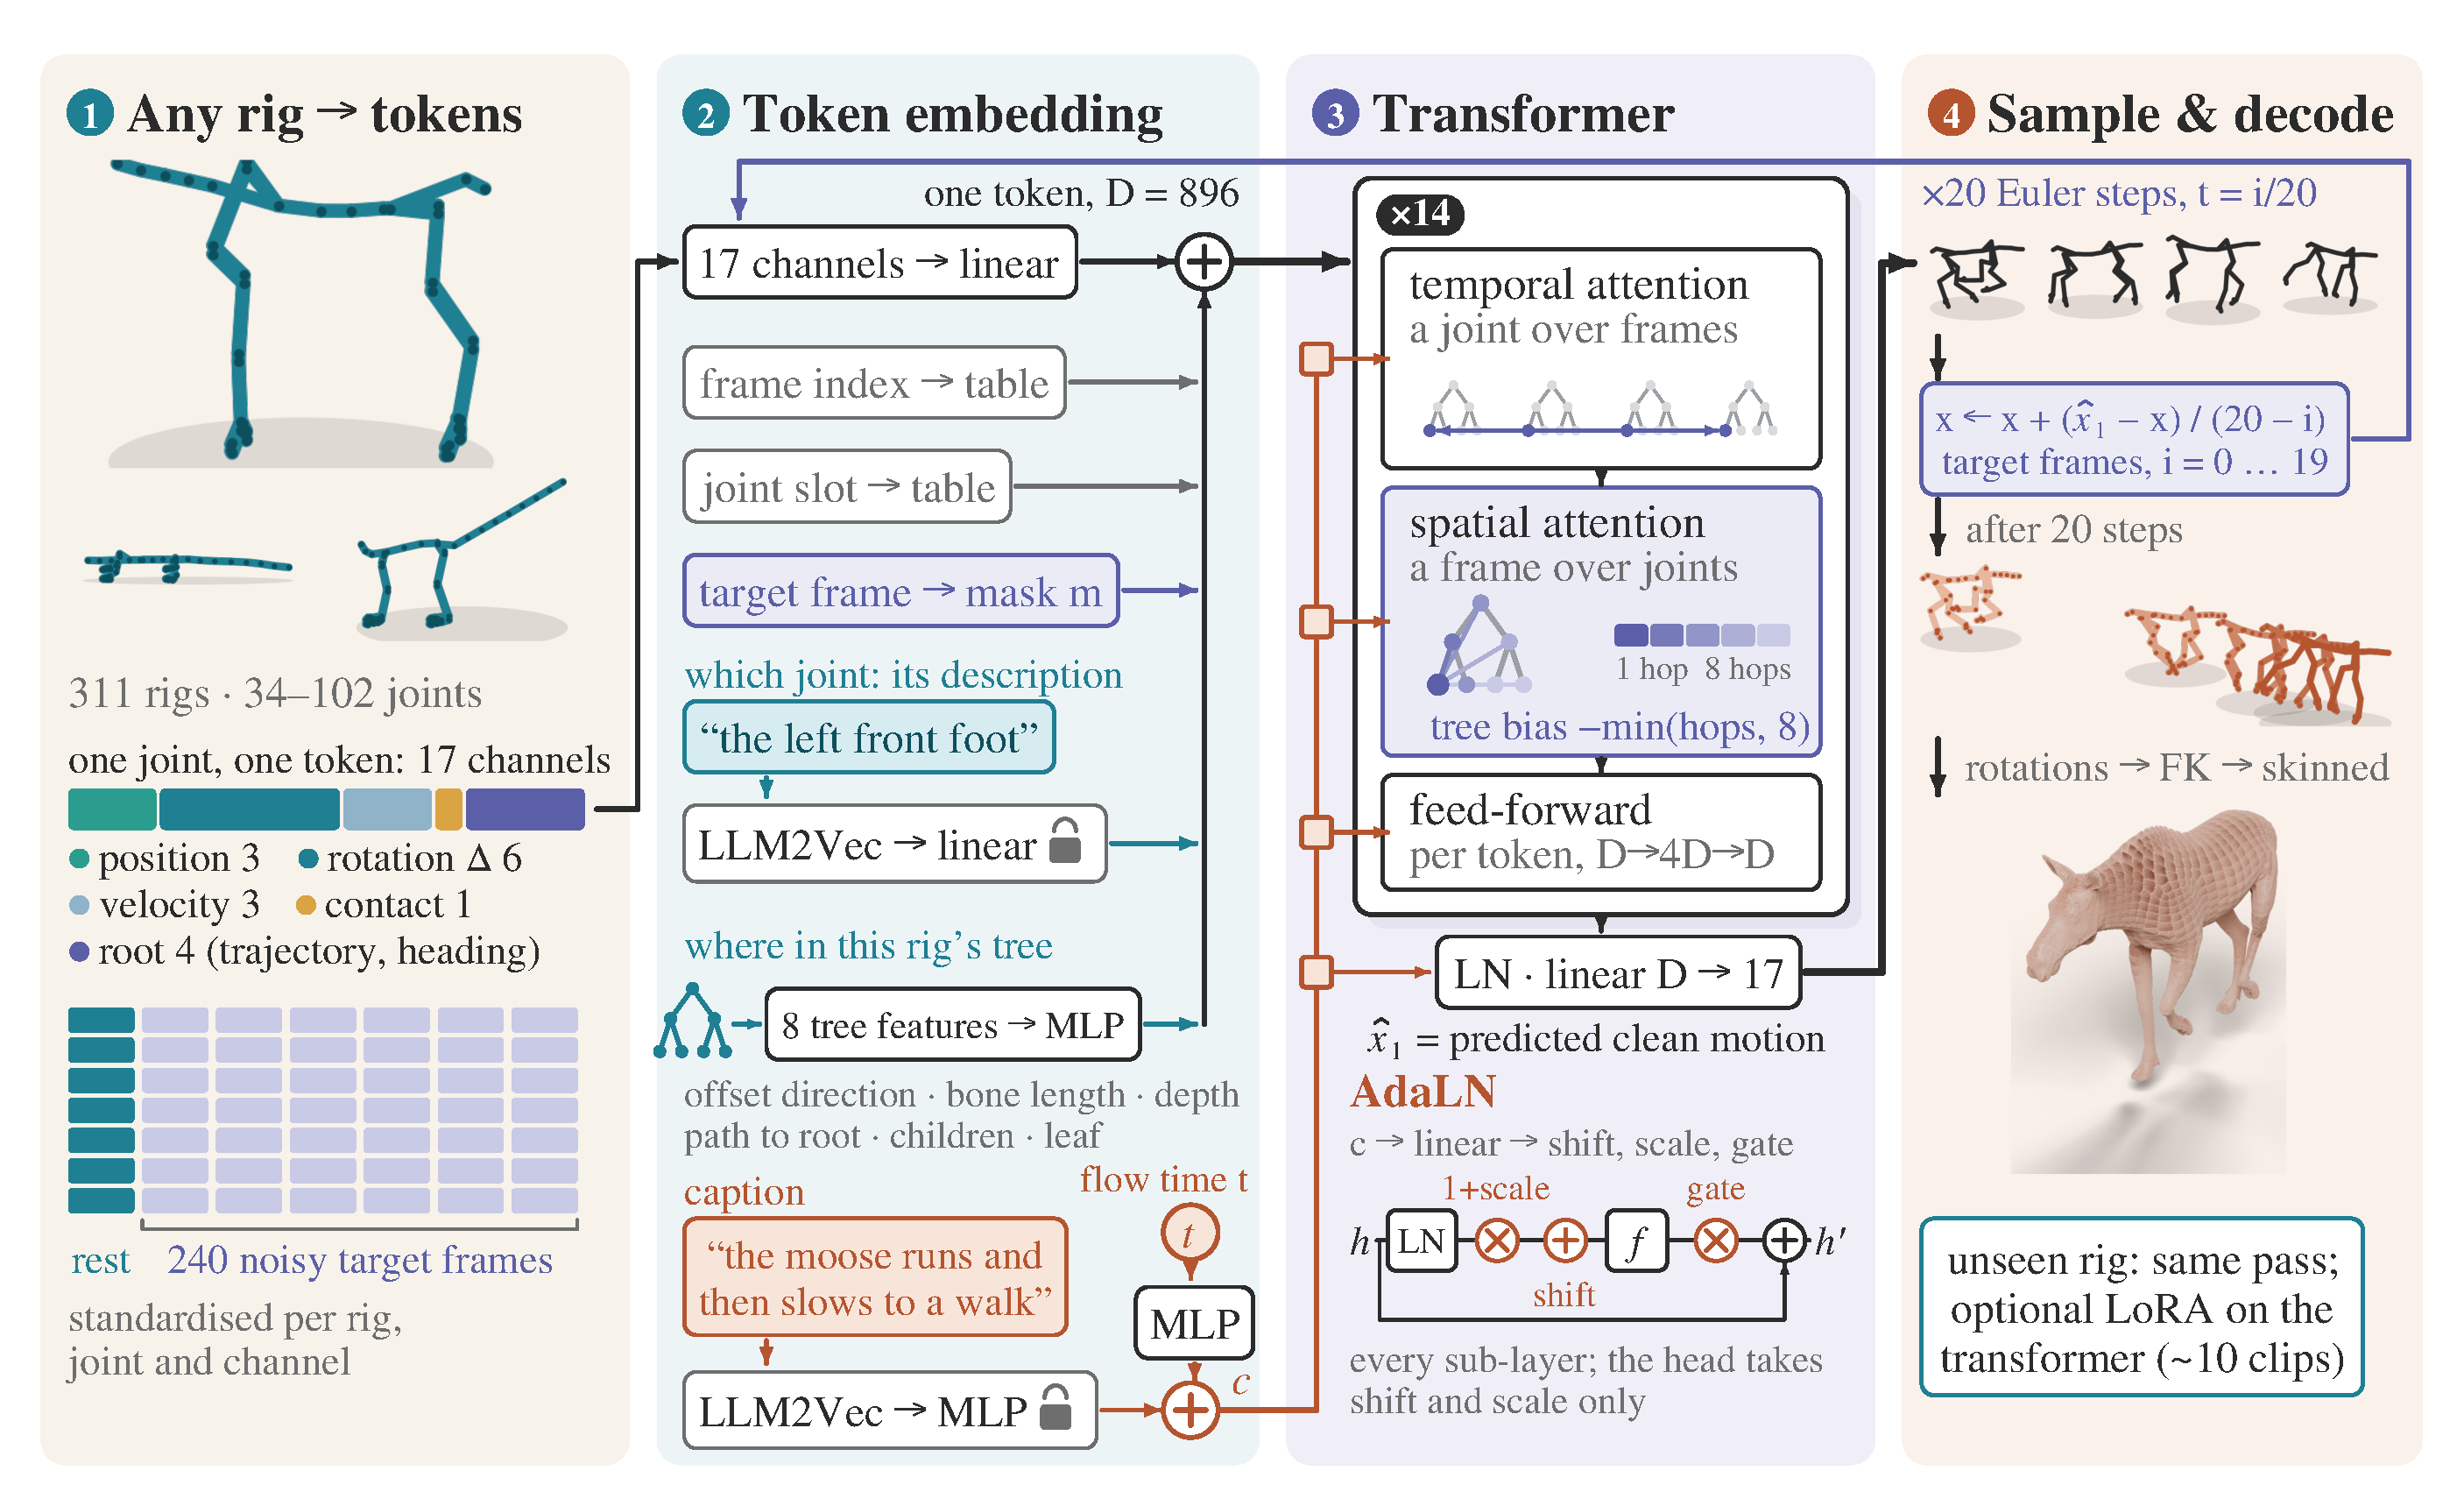
\includegraphics[width=\linewidth]{figures/fig1_align/figure1.pdf}
\caption{\method{} overview. A rig enters as data: each joint of each frame is one token of 17 standardised channels, and the
sequence is the rig's clean rest pose followed by 240 noise-mixed target frames. A token is the sum of six terms (band~2). The caption
and the flow time form $\mathbf c$, which sets the shift, scale and gate of every sub-layer (AdaLN) and is the caption's only route
into the network. Fourteen blocks alternate temporal and spatial attention, the latter biased by tree distance; the head predicts the
clean motion $\hat{\mathbf x}_1$, and 20 Euler steps with caption guidance $s{=}2$ update the target frames only; rotations are then
forward-kinematised on the rig and skinned. An unseen rig takes the same pass, optionally with a ten-clip LoRA. All glyphs are the
model's own output on a moose run-to-walk clip.}\label{fig:teaser}
\end{figure}

The applications that most need generative motion---games, film
previsualisation, virtual production---are populated by characters that are
emphatically not human: quadrupeds with digitigrade gaits, reptiles that
sprawl, birds with wing chains, animals with tails, trunks and shells. A studio
does not have one skeleton; it has hundreds, each authored by a rigger with its
own joint count, naming scheme and helper bones. The corpus we train on is a
faithful sample of that reality: \num{311} production animal rigs with
\num{34} to \num{102} deformation joints (median 64), \num{108} distinct kinematic trees, and
\num{77{,}894} captioned clips (\num{6.2}M frames).\footnote{The rigs and animations are
re-exported from the assets of a commercial zoo-management game, deformation bones only; the assets
are used for research and are not redistributed (App.~\ref{app:rep}). The Truebones zoo, a publicly
distributed set of 66 animal rigs, is kept entirely outside training and serves as the held-out
test of skeletons the model has never seen.}

Two workarounds exist, and both are unsatisfying: a model per character multiplies data and
compute by the size of the cast and fails for characters with a handful of clips, and generating
on a canonical skeleton and \emph{retargeting}~\citep{villegas2018nkn,aberman2020skeleton,lee2023same}
degrades as morphology diverges---it is unclear what it would even mean to transfer a walking human
to a tortoise. The motion has to be generated for the target body.

\paragraph{Our position.} A generative model should treat the skeleton as \emph{input}, not as
architecture: if the network is told the kinematic tree, the rest pose and what each joint \emph{is}
at inference time, adding a character becomes a data question. The analogy is speech: F5-TTS
\citep{chen2024f5tts} clones a voice from seconds of reference audio placed in context while the
transcript says what to say; the reference audio of a \emph{body} is a single frame, its rest pose,
and the caption says what the body should do. The interface itself is due to
AnyTop~\citep{gat2025anytop}, which prepends the rest pose as a first frame and
adds joint-name embeddings to generate, without text, for the Truebones zoo;
text-conditioned animal generation has since been studied on 140 species by
OmniZoo~\citep{chen2025omnizoo}, on a shared topology by X-MoGen~\citep{wang2025xmogen}
and on Truebones by G-MDM~\citep{lee2025dragon} and SAMoR~\citep{samor2026}.
What has not been shown is how far one text-conditioned model stretches across
hundreds of heterogeneous \emph{production} rigs denoised in their own
per-joint space, what it takes to train it at 0.3B parameters, and how cheaply
it can be \emph{extended} to a body it has never seen.

\paragraph{\method{}.} We answer these questions with four design choices.
\begin{enumerate}[leftmargin=*,itemsep=1pt,topsep=2pt]
\item \textbf{A per-joint motion representation with per-rig normalisation}
  (\rep{}, Section~\ref{sec:method:rep}): every joint carries the same 17
  channels (position, rotation as a 6D delta from the rest pose, velocity,
  contact, plus root-only trajectory and heading), and every (rig, joint,
  channel) cell is normalised with its own statistics, so hundreds of rigs with
  different proportions, joint counts and conventions share one network input.
\item \textbf{In-context skeleton conditioning}
  (Section~\ref{sec:method:model}): the target skeleton is presented to a
  diffusion transformer as a one-frame \emph{rest-pose} prompt prepended to
  the sequence, together with embeddings of natural-language descriptions of
  its joints (``left front lower leg'', ``tail segment 3'') and a
  graph-distance attention bias. The prompt follows AnyTop; we replace joint
  names by descriptions, add text control, and denoise the raw per-joint
  representation, so no joint vocabulary, joint ordering or per-skeleton
  parameter is baked into the architecture.
\item \textbf{A calibrated grouped flow-matching objective}
  (Section~\ref{sec:method:objective}): channel groups (root and body
  position, rotation, velocity, contact, trajectory, heading) are weighted from
  measured group energies so that the root, contact and trajectory channels of
  a large rig are not drowned by its many body rotations; a mechanism check on
  the pilot model verifies the implementation before training, and
  forward-kinematics, contact and acceleration terms are added in the same
  frame.
\item \textbf{Extensibility to unseen bodies from a handful of clips}
  (Section~\ref{sec:method:lora}): because the model denoises the raw
  per-joint representation and carries no skeleton-specific parameters, a rig
  it has never seen is served by the same forward pass once its rest pose,
  joint descriptions and per-cell statistics are supplied, and a per-rig LoRA
  trained on roughly ten clips adapts it to bodies far outside the training
  distribution (a winged dragon, an eight-legged spider).
\end{enumerate}

\paragraph{Results.} A single \num{303}M-parameter \method{} trained on all \num{311} rigs is
scored by a skeleton-aware text--motion evaluator on \num{3{,}899} held-out clips: R@1 \num{0.922}
against \num{0.964} for the real clips, FID \num{0.005} (\S\ref{sec:exp:main}). Query--key normalisation
made the 0.3B model trainable in our runs. On Truebones rigs never seen in training the frozen
backbone moves, but with \num{2.5} to \num{13} times the jitter of the real clips; a per-rig LoRA on
ten to fifteen clips lowers the validation FK--pose gap---the disagreement between the rotation and
position channels of the denoiser's prediction---by \num{59}\% on a buffalo and from \num{1.215}
to \num{0.146} bone lengths on a 95-joint dragon, while the adapted outputs move less than the real
clips; an adapter shared by eight flying rigs is \emph{worse} than the species-specific one. On the
same rigs we report descriptive kinematic statistics next to the released AnyTop
model~\citep{gat2025anytop}, which trained on them, as an in-distribution reference. Every
retrieval number is reported next to the evaluator's score on real motion.

\paragraph{Contributions.} (i) \emph{Data.} \rep{}, a per-joint representation any rigged
animation converts to from its kinematic tree, rest pose and motion, with no template, retargeting
or tokenizer, and the captioned corpus of \num{311} production animal rigs built with it.
(ii) \emph{A framework for many topologies.} \method{}, a text-to-motion diffusion transformer
serving hundreds of skeletons with one set of weights, with the objective and recipe that trained
it at 0.3B (calibrated grouped loss, qk-normalised attention, spike rejection).
(iii) \emph{Extensibility.} A rig never seen is served by the same forward pass once its statistics
are supplied, and a low-rank adapter trained on eight to twenty-six clips extends the model to bodies far outside the training
distribution, quantified with the FK--pose gap and descriptive kinematics in a study of per-rig and
cross-species adapters with a negative result on sharing.
